\documentclass[12pt,a4paper]{report}

% Packages
\usepackage[margin=1in,left=1.5in]{geometry}
\usepackage{times}
\usepackage{setspace}
\usepackage{titlesec}
\usepackage[nottoc,notlot,notlof]{tocbibind}
\usepackage{tocloft}
\usepackage{fancyhdr}
\usepackage{graphicx}
\usepackage{booktabs}
\usepackage{usecase}
\usepackage{xcolor}
\usepackage{hyperref}

% hide links so no color appear, but they still work :D
\hypersetup{
    hidelinks
}

% Page numbering
\pagenumbering{roman}

% Title formatting
\titleformat{\chapter}{\normalfont\huge\bfseries\uppercase}{\thechapter}{20pt}{\huge}

% Document begin
\begin{document}

% Title Page
\begin{titlepage}
    \begin{center}
        \vspace*{1cm}
        
\includegraphics[height=1cm]{images/yu-logo.png}\\[1cm]
        {\Large\bfseries AL YAMAMAH UNIVERSITY}\\[0.5cm]
        {\large College of Engineering and Architecture}\\[0.5cm]
        {\large Bachelor of Science in Software and Network Engineering}\\[2cm]
        {\Huge\bfseries 
            \begin{spacing}{1}
                Jadwal: An Elegant, iOS-based Calendar Manager
            \end{spacing}
        }
        \vspace{2cm}
        {\Large\bfseries Graduation Project}\\[2cm]
        \begin{center}
            \setlength{\fboxsep}{10pt}
            \setlength{\fboxrule}{1pt}
            \fbox{
                \begin{tabular}{p{0.45\linewidth}p{0.45\linewidth}}
                    \multicolumn{2}{c}{\textbf{Group Project Submission}} \\
                    \midrule
                    \textbf{Student Names} & \textbf{Student IDs} \\
                    \midrule
                    YAZED ALKHALAF & 202211123 \\
                    SAIMAN TAKLAS & 202021400 \\
                    AFFAN MOHAMMAD & 202211086 \\
                    ALI BA WAZIR & 202211018 \\
                    \midrule
                    \multicolumn{2}{l}{\textbf{Submission Date}: 19 Sep 2024} \\
                    \multicolumn{2}{l}{\textbf{Supervised By}: Dr. Inaya Allah} \\
                \end{tabular}
            }
        \end{center}
        \vfill
        {\large First Semester 2024--2025}
    \end{center}
\end{titlepage}

% Preface section
\chapter*{Abstract}
\addcontentsline{toc}{chapter}{Abstract}

\chapter*{Acknowledgment}
\addcontentsline{toc}{chapter}{Acknowledgment}
\newpage

\tableofcontents

\newpage
\listoffigures

\newpage
\listoftables
\newpage

\chapter*{List of Abbreviations}
\addcontentsline{toc}{chapter}{List of Abbreviations}

% Main body (switch to Arabic numerals)
\pagenumbering{arabic}

\chapter{Introduction}


\section{Background of the Study}

As the world is moving towards globalizing, effective time management is becoming very important. Considering how everything seems to be rushing in today's world, there is a high requirement for an effective user-friendly time management tool. Paper-based calendars have been used for addressing the complexities of managing multiple schedules across various aspects of life such as work, school, and personal commitments. However, they often fall short in providing a comprehensive solution to modern scheduling challenges.

The introduction of the digital calendar has somewhat solved this problem but still, users face a lot of issues in keeping their calendars up-to-date and synchronized. There are still few people that manually input events into their calendars. This could be really tiring, especially when dealing with multiple calendars.

Moreover, the rise of instant messaging platforms like WhatsApp has changed the way we communicate and plan events. Mostly, important dates and appointments are discussed informally leading to a disconnect between where the information is initially shared and where it needs to be recorded for effective time management.

To address these challenges, we are planning an application called \textit{Jadwal}, which aims to revolutionize how people manage their time and schedules in the digital age.

\section{Problem Statement}

Users often face challenges in keeping their calendars up-to-date, particularly when dealing with information from various sources, including informal communication mediums like WhatsApp. The process of manually adding events to the calendar is both time-consuming and prone to errors. Additionally, managing multiple calendars—such as those for work, school, and personal life—creates further complexity and increases the risk of scheduling conflicts. The lack of seamless integration with popular communication platforms exacerbates the problem, leading to a higher likelihood of missing important events due to the scattered distribution of information across different calendars and data sources.

\section{Objectives of the Study}

The main objectives of Jadwal are:

\begin{itemize}
    \item To develop an intelligent calendar management system that automatically extracts events from the communication channels and adds them to the user's main calendar.
    \item To create a user friendly interface that allows users to automatically add events to the calendar.
    \item To implement smart resolution system that notifies users of scheduling conflicts and provides easy options for resolution.
    \item To integrate all the calendars into Jadwal's single calendar view to make viewing and managing all the events easy.
    \item To prioritize and automatically schedule daily routines such as waking time, sleeping time and prayer time.
    \item To significantly reduce the time users spend on manual calendar management.
\end{itemize}

\section{Scope of the Study}

Jadwal is not just another calendar application; it's a comprehensive time management tool designed to aggregate and optimize your existing calendars and data sources. The scope of the project includes:

\begin{itemize}
    \item Development of an iOS application as the primary platform.
    \item Integration with calendars using CalDAV.
    \item WhatsApp message parsing for event extraction (subject to technical feasibility).
    \item Target audience: Busy professionals, students, and anyone juggling multiple schedules.
    \item User testing phase to ensure ease of use and effectiveness.
\end{itemize}

Our testing methods will include:
\begin{itemize}
    \item Beta testing with a diverse group of users.
    \item Analytics to track user behavior and app performance.
\end{itemize}

\section{Significance of the Study}

Jadwal endeavours to solve problems and its significance can be summarized in the following:

\begin{enumerate}
    \item \textbf{Time is Money}: Time is the only asset you can't get more of, it is being consumed til the last day of your life.
    \item \textbf{Prayer First Calendar}: Prayer times come first, then your daily scheduled items.
    \item \textbf{Streamlined Time Management}: By automatically extracting events from various communication channels, Jadwal significantly reduces the time and effort required for manual calendar management, allowing users to focus on more productive tasks.
    \item \textbf{Reduced Human Error}: Automated event extraction and addition to calendars minimize the risk of missing important events or appointments due to manual input errors or forgetfulness.
    \item \textbf{Integrated Communication and Scheduling}: By bridging the gap between informal communication (e.g., WhatsApp) and formal scheduling, Jadwal addresses a critical pain point in modern time management.
    \item \textbf{Conflict Resolution}: The smart resolution system helps users identify and resolve scheduling conflicts efficiently, reducing stress and improving overall time management.
    \item \textbf{Holistic View of Commitments}: By integrating multiple calendars into a single view, Jadwal provides users with a comprehensive overview of their commitments across various aspects of life, facilitating better decision-making and work-life balance.
\end{enumerate}

\section{Limitations of the Study}

Nothing is perfect, and our project is not a outlier. The limitations we have figured out about it are as follows:

\begin{itemize}
    \item WhatsApp integration allows the app to read the users messages, so it would be hard to prove privacy hasn't been breached.
    \item WhatsApp integration might not always be there, they are a third-party.
    \item Learning new technologies for iOS development might require more time than anticipated.
    \item Accuracy of our algorithms to detect keywords indicating an event agreement has happened, especially for languages other than English.
    \item Time and manpower constraints may limit the number of features we can implement.
    \item Dependency on third-party calendar APIs and their limitations.
\end{itemize}

\section{Organization of the Senior Project}

Our project plan can be illustrated in the following gantt chart, \textbf{Figure \ref{fig:project-gantt-chart}}.

\begin{figure}[!h]
    \centering
    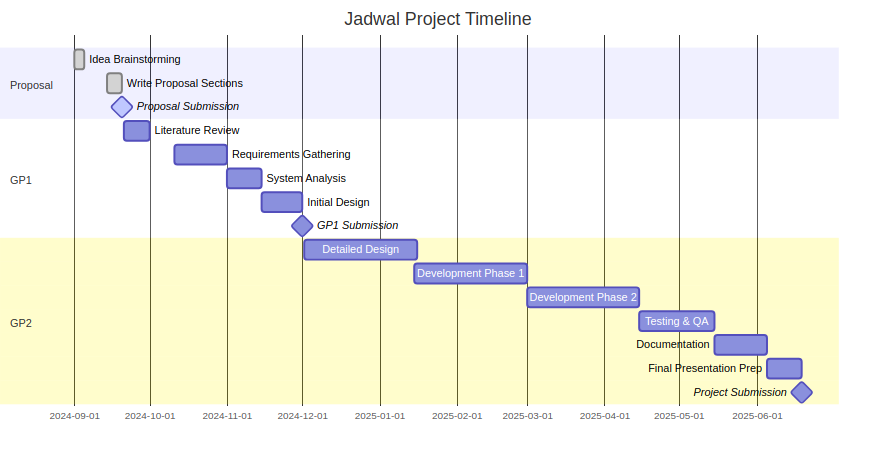
\includegraphics[width=\textwidth]{images/gantt.png}
    \caption{Project Gantt Chart}
    \label{fig:project-gantt-chart}
\end{figure}

\chapter{Literature Review}

In developing Jadwal, we have drawn inspiration from and built upon existing research and products in the field of intelligent calendar management. Some key references include:

\begin{itemize}
    \item \textbf{Clockwise (https://www.getclockwise.com/):} A smart calendar assistant that optimizes schedules and manages team coordination \cite{clockwise}. Clockwise's approach to intelligent time blocking and meeting optimization provides valuable insights for Jadwal's automated scheduling features.
    \item \textbf{Motion (https://www.usemotion.com/):} Motion's Intelligent Calendar takes your meetings, your tasks, your to-do list, your activities, and creates one perfect, optimized schedule to get it all done \cite{motion}.
    \item \textbf{Reclaim AI (https://reclaim.ai/):} An intelligent time management tool that helps optimize schedules and automate tasks \cite{reclaim}.
    \item \textbf{Calendi (https://calendi.ai/):} Calendi describes itself as: ``Calendi is an AI calendar system. Use it for scheduling tasks, automating meetings, and witness the future of calendar.'' \cite{calendi}
    \item \textbf{An Exploratory Study of Calendar Use:} ``Prospective remembering is the use of memory for remembering to do things in the future, as different from retrospective memory functions such as recalling past events.'' \cite{tungare2008exploratorystudycalendaruse}
    \item \textbf{WhatsApp Integration:} Our research indicates that direct WhatsApp integration for event extraction has not been widely implemented in existing calendar applications, making this a unique feature of Jadwal.
\end{itemize}

\begin{figure}[!h]
    \centering
    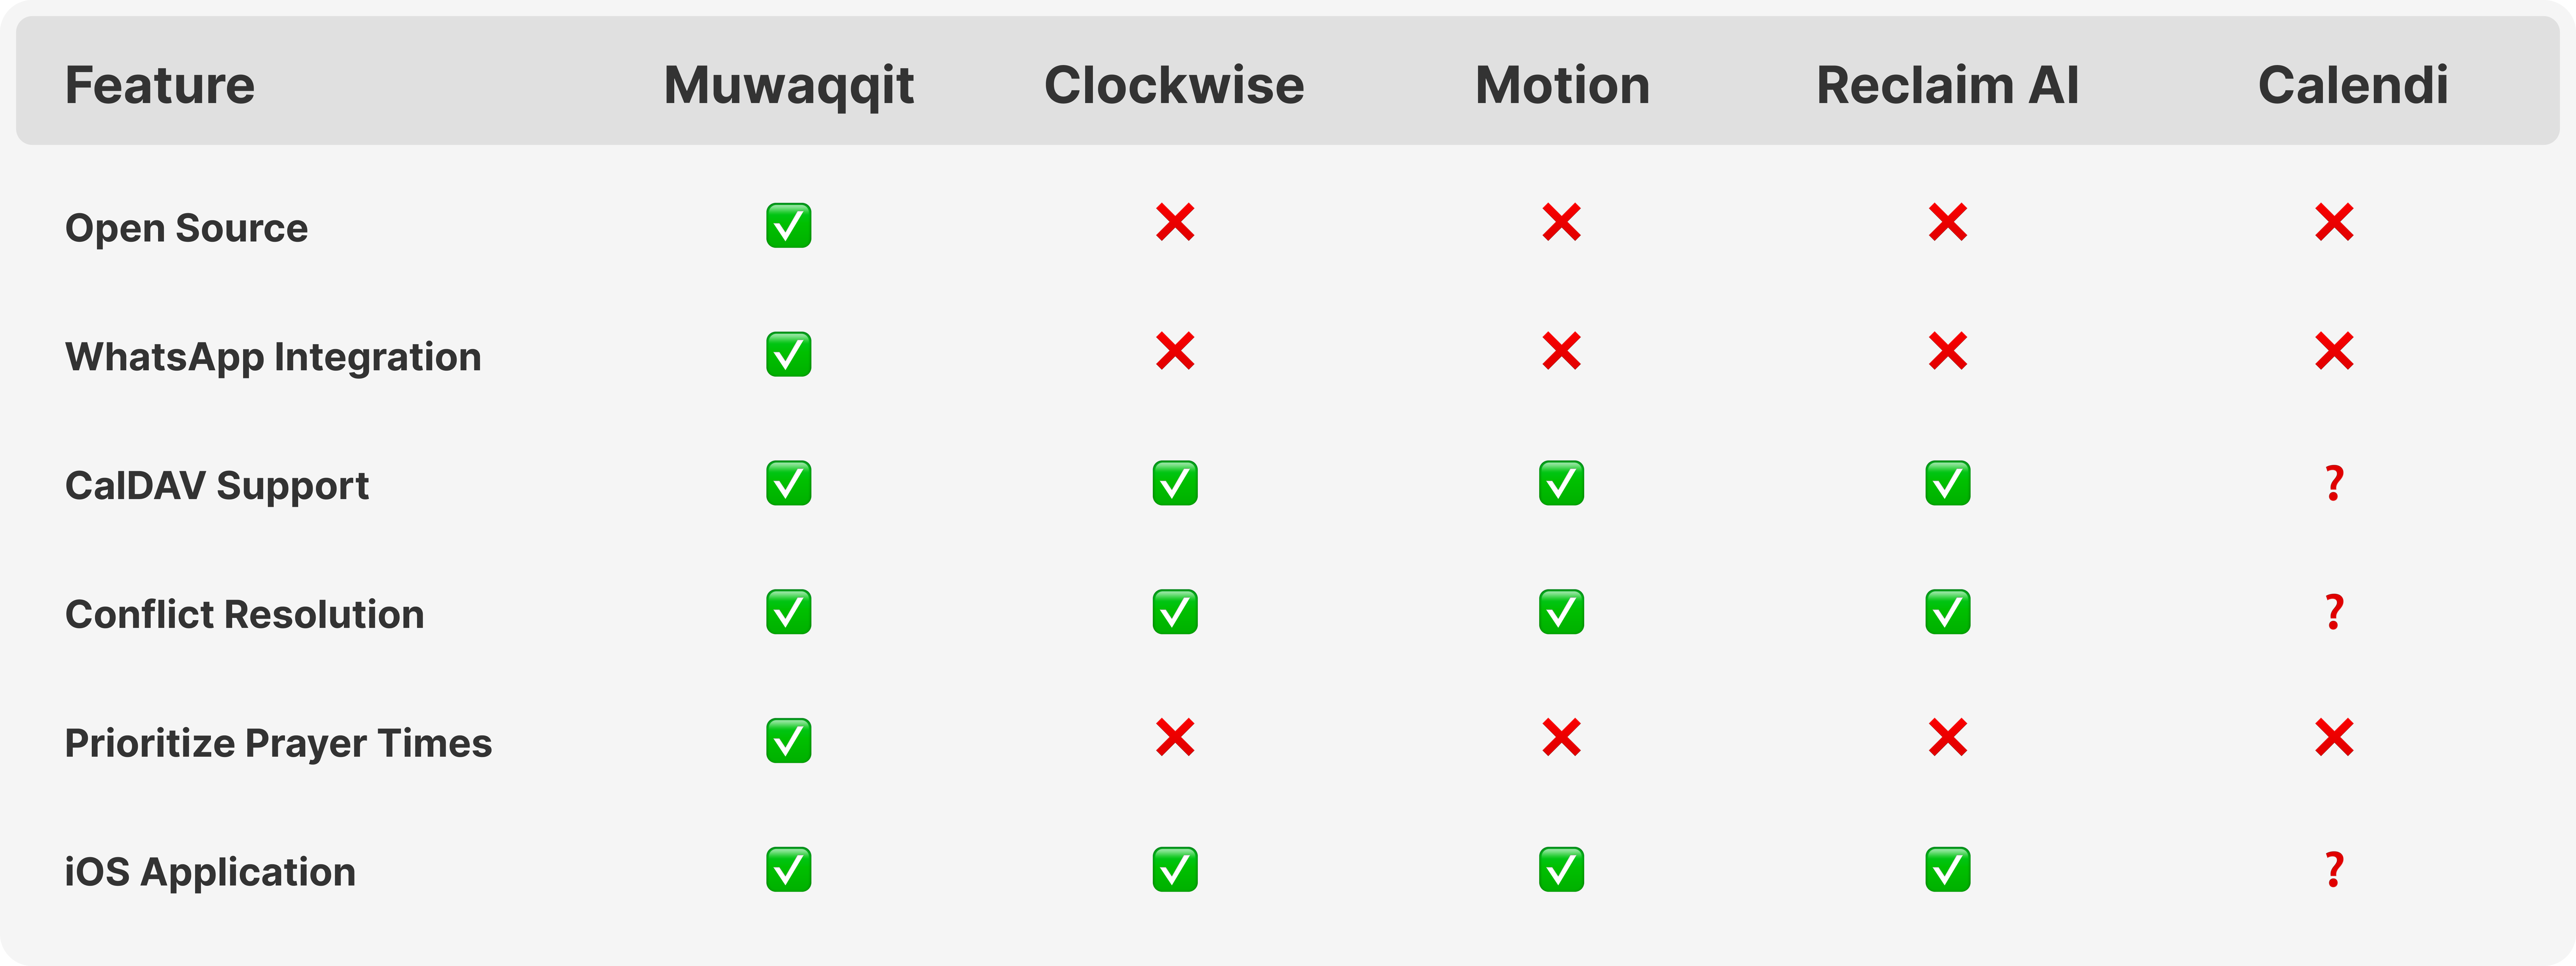
\includegraphics[width=\textwidth]{images/features-table.png}
    \caption{Feature Comparison Table}
    \label{fig:features-table}
\end{figure}

\chapter{System Analysis and Design}

\section{Functional Requirements}

\begin{itemize}
    \item The user shall be able to access their account using either Google OAuth or magic link via Email. For new users, a new accout is created, and for existing users, they are given access to their account directly
    \item The system shall send a welcome email to new users.
    \item The user should be able to connect a calendar using CalDAV.
    \item The user should be able to connect their WhatsApp account.
    \item The user should be able to add events manually and set priorities optionally.
    \item The user should be able to view integrated calendar.
    \item The user should be able to configure daily routines.
    \item The user should be able to manage scheduling conflicts.
    \item The user should be able to schedule prayer times.
    \item The system shall send event notifications to the user.
    \item The system shall personalize the experience based on answers provided by the users.
    \item The system shall add the WhatsApp extracted events to the calendar. If a conflict occurs, the user shall get a notification to resolve the conflict with suggestions.
    \item The system shall synchronize calendar data across multiple devices.
\end{itemize}

\section{Non-Functional Requirements}

\begin{itemize}
    \item \textbf{Platform Compatibility:} The app shall be compatible with iOS devices running iOS 14.0 or later.
    \item \textbf{Performance:} The app shall load the main calendar view within 3 seconds on 5G with speeds above 200mpbs.
    \item \textbf{User Experience:} The user interface shall follow iOS Human Interface Guidelines for consistency and ease of use.
    \item \textbf{Security:} All data transmissions between the app and servers shall be encrypted using HTTPS.
    \item \textbf{Localization:} The app shall support localization in Arabic and English.
    \item \textbf{Data Privacy:} The app shall comply with the data protection regulations and laws in Saudi Arabia.
\end{itemize}

\section{System use-cases}

\textbf{Figure \ref{fig:use-case-diagram}} shows the use case diagram for the system of Jadwal.

\begin{figure}[!h]
    \centering
    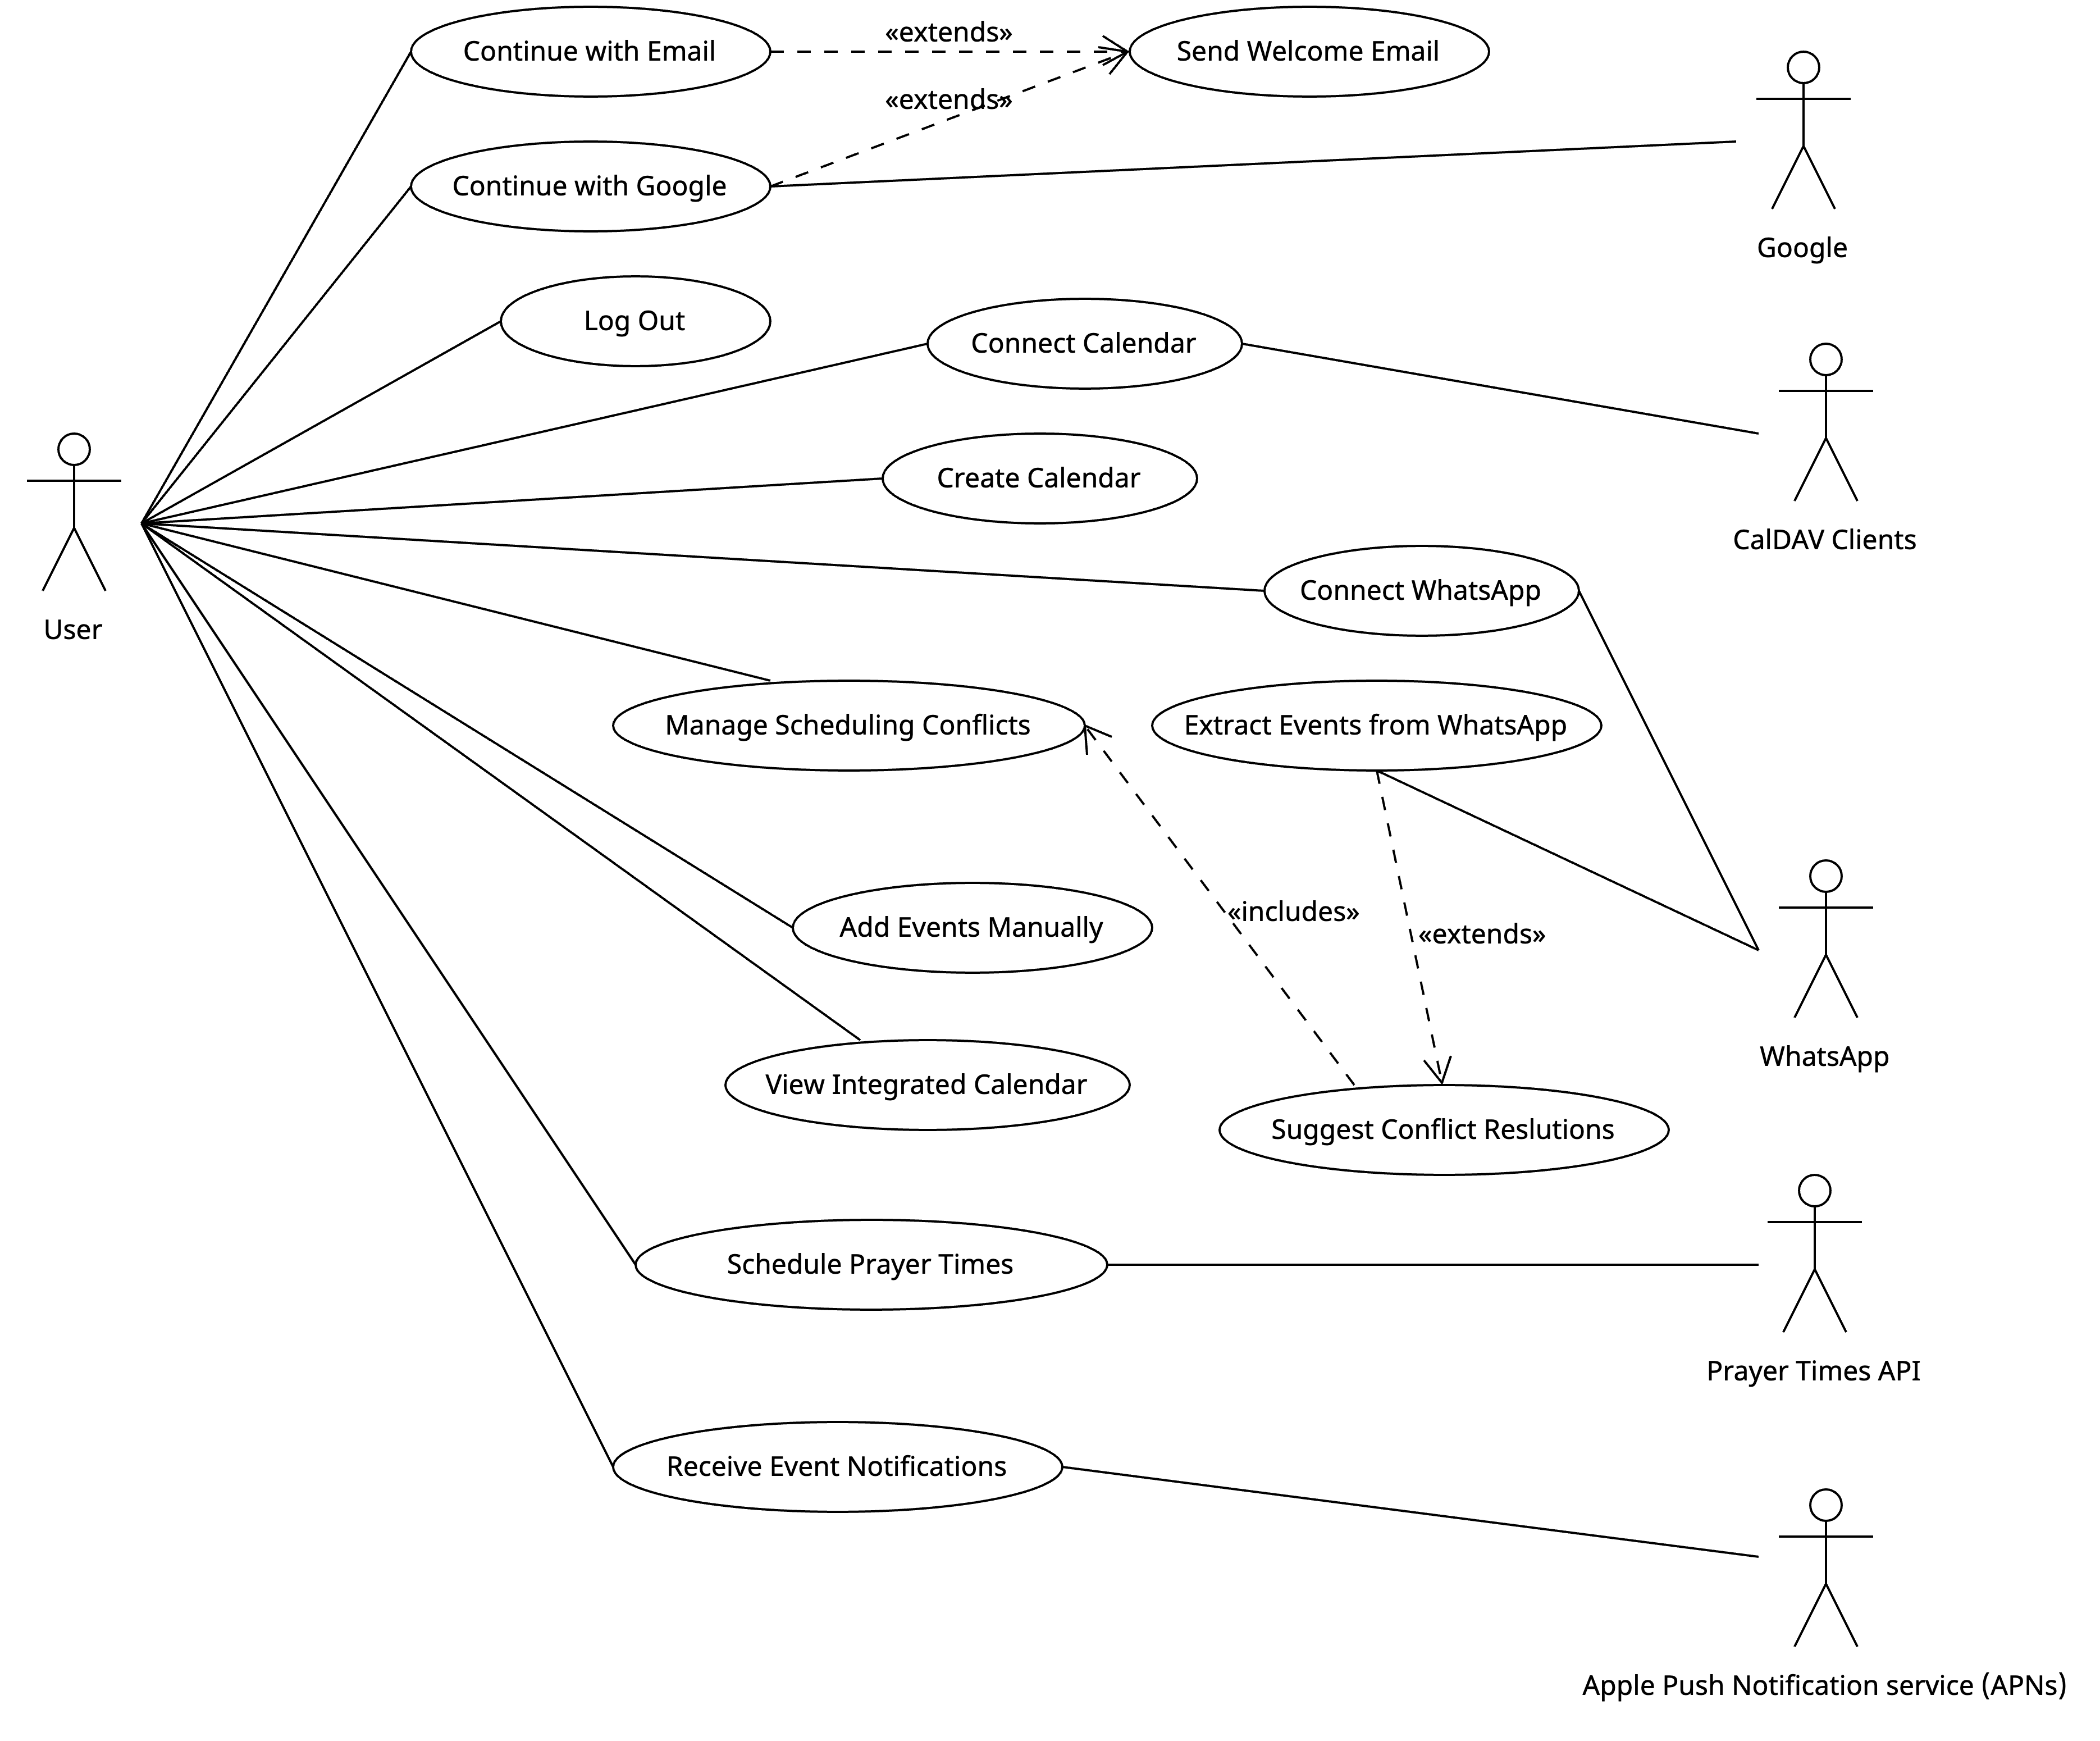
\includegraphics[width=\textwidth]{images/use-case-diagram.png}
    \caption{Use Case Diagram of Jadwal}
    \label{fig:use-case-diagram}
\end{figure}

\begin{usecase}{Continue with Email}
  \ucbasicinfo{High}{Regular}
  \ucshortdescription{This UC allows users to login or create an account using their email.}
  \uctrigger{This UC starts when the user enters their email to the system.}
  \ucactors{User}{None}
  \ucpreconditions{User must have an email}
  \ucrelationships{Send Welcome Email}{N/A}{N/A}
  \ucinputsoutputs{
    \begin{itemize}
      \item \textbf{Email} (Source: User)
      \item \textbf{Magic Link (from email)} (Source: User)
    \end{itemize}
  }{
    \begin{itemize}
      \item \textbf{Magic link email} (Destination: User)
      \item \textbf{Confirmation messages} (Destination: User Interface)
      \item \textbf{JWT} (Destination: App)
    \end{itemize}
  }
  \ucmainflow{
    \begin{enumerate}
      \item The user enters their email.
            \ucinfo{System displays an email input field.}
      \item System creates an account if the user has no account, and then generates and sends the magic link.
            \ucinfo{App displays ``Check your email'' message.}
      \item The user clicks the magic link in the email.
            \ucinfo{The app is opened on the device of the user.}
      \item The app sends the token to the system to log the user in.
            \ucinfo{System verifies token and logs user in.}
    \end{enumerate}
  }
  \ucalternateflows{
    \begin{itemize}
      \item The user cancels the authentication request.
    \end{itemize}
  }
  \ucexceptions{
    \begin{itemize}
      \item Invalid email format.
      \item Magic link token expired or invalid.
      \item \textbf{Request sending failure}: If sending the request fails due to network issues, the system prompts the user to try again.
    \end{itemize}
  }
  \ucconclusion{This UC ends when the user is logged in.}
  \ucpostconditions{The system generates a JWT.}
  \ucspecialrequirements{An email server must be present to send magic link email.}
\end{usecase}

\begin{figure}[!h]
  \centering
  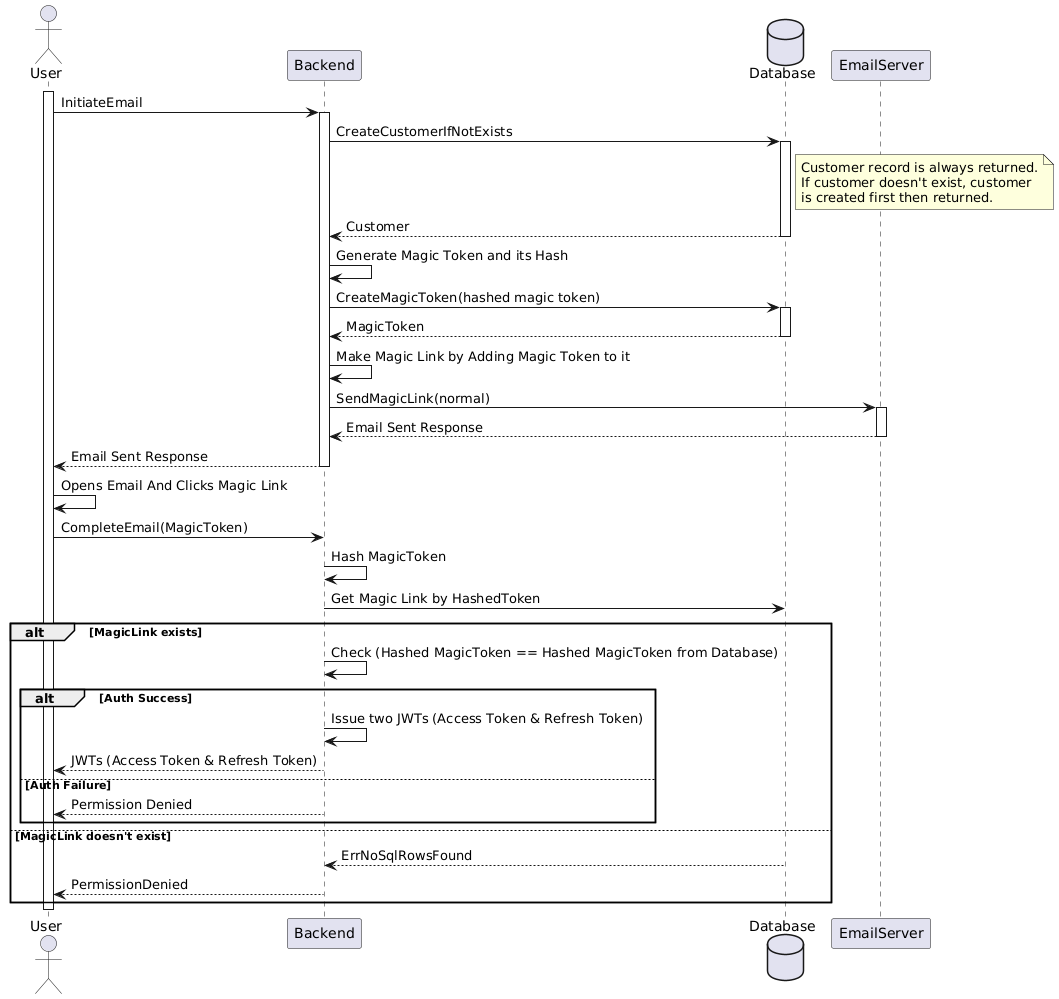
\includegraphics[width=\textwidth]{images/docs/diagrams/sequence-diagrams/all-sequence-diagrams/Continue with Email.png}
  \caption{Continue with Email Sequence Diagram}
  \label{fig:seq/continue-with-email}
\end{figure}

The "Continue with Email Sequence Diagram", shown in \textbf{Figure~\ref{fig:seq/continue-with-email}}, illustrates the process of email-based magic link authentication, involving interactions between the User, Backend, Database, and EmailServer. The process begins when the user initiates an action, such as signing up or logging in. The backend executes the CreateCustomerIfNotExists function to retrieve an existing customer record or create a new one if none exists. Once the customer is identified, the backend generates a magic token and its hashed version using the GenerateMagicToken function. The hashed token is stored in the database, and a magic link containing the token is created. The backend then sends the magic link to the user's email using the SendEmail function via the email server. The user clicks the magic link, triggering the CompleteFlow(MagicToken) request to the backend, where the provided token is validated against the stored hashed token in the database. If the tokens match, authentication succeeds, and the backend issues a JSON Web Token (JWT) to the user for future access. In cases where the token is invalid, expired, or the customer record is missing, the system responds with appropriate errors, such as PermissionDenied or EntryNotFound. This diagram demonstrates a secure flow for handling authentication via email magic links.
\begin{usecase}{Continue with Google}
  \ucbasicinfo{High}{Regular}
  \ucshortdescription{This UC allows users to login or sign up with their Google account.}
  \uctrigger{This UC starts when the user clicks ``Continue with Google'' button in the app.}
  \ucactors{User}{Google}
  \ucpreconditions{The user must have an active Google account.}
  \ucrelationships{Send Welcome Email}{N/A}{N/A}
  \ucinputsoutputs{
    \begin{itemize}
      \item \textbf{Google access token} (Source: User)
    \end{itemize}
  }{
    \begin{itemize}
      \item \textbf{Authentication response} (Destination: User)
      \item \textbf{JWT} (Destination: App)
    \end{itemize}
  }
  \ucmainflow{
    \begin{enumerate}
      \item The user click continue with Google.
        \ucinfo{App uses OAuth to authenticate with Google}
      \item App sends Google access token to the system.
        \ucinfo{System verifies the token is issued for us and then issues JWT for usage within the app.}
    \end{enumerate}
  }
  \ucalternateflows{
    \begin{itemize}
      \item The user cancels the authentication request.
    \end{itemize}
  }
  \ucexceptions{
    \begin{itemize}
      \item Google access token invalid or expired.
      \item \textbf{Request sending failure}: If sending the request fails due to network issues, the system prompts the user to try again.
    \end{itemize}
  }
  \ucconclusion{This UC ends when the user is logged in.}
  \ucpostconditions{The system generates a JWT.}
  \ucspecialrequirements{A google client must be present for the validation of the access token to be possible.}
\end{usecase}

\begin{figure}[!h]
  \centering
  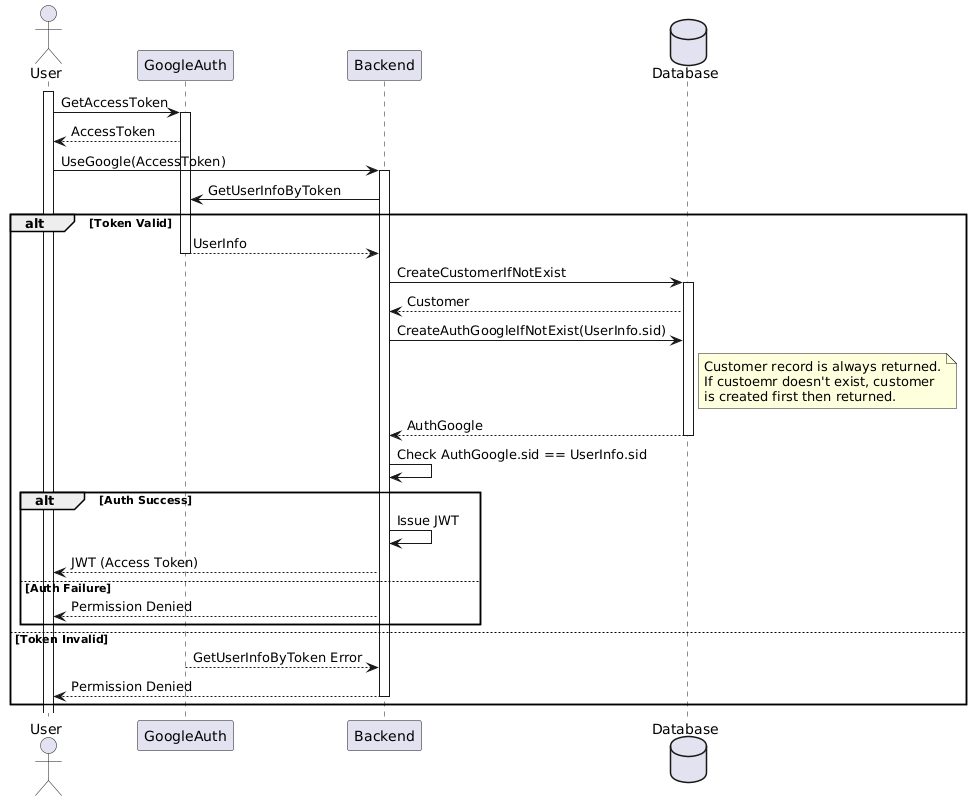
\includegraphics[width=\textwidth]{images/docs/diagrams/sequence-diagrams/all-sequence-diagrams/Continue with Google.png}
  \caption{Continue with Google Sequence Diagram}
  \label{fig:seq/continue-with-google}
\end{figure}
\begin{usecase}{Connect WhatsApp}
  \ucbasicinfo{Medium}{Regular}
  \ucshortdescription{This UC allows the user to connect their WhatsApp account to the system.}
  \uctrigger{This UC is triggered when the user clicks on ``Connect WhatsApp'' button in the app.}
  \ucactors{User}{WhatsApp}
  \ucpreconditions{User must be logged in}
  \ucrelationships{N/A}{N/A}{N/A}
  \ucinputsoutputs{
    \begin{itemize}
      \item \textbf{WhatsApp phone number} (Source: User)
      \item \textbf{WhatsApp linking code} (Source: User)
    \end{itemize}
  }{
    \begin{itemize}
      \item \textbf{WhatsApp auth credentials} (Destination: System)
    \end{itemize}
  }
  \ucmainflow{
    \begin{enumerate}
      \item The user clicks ``Connect WhatsApp'' button.
            \ucinfo{The system asks for the user's WhatsApp phone number.}
      \item The user enters their WhatsApp phone number.
            \ucinfo{WhatsApp shows the linking code in their app.}
      \item The user enters the linking code in our app.
            \ucinfo{The app shows a success screen if connection was sucessful.}
    \end{enumerate}
  }
  \ucalternateflows{
    \begin{itemize}
      \item If the WhatsApp connection fails, the user must redo the steps and try again.
      \item If the user enters a wrong linking code, the connection of the WhatsApp account will fail unless they enter the correct code.
    \end{itemize}
  }
  \ucexceptions{
    \begin{itemize}
      \item \textbf{Wrong linking code:} If the user enters a wrong linking code too many times, the connection of the WhatsApp account will fail.
      \item \textbf{Network issue:} A network issue interrupting the communication between the app, the server, and WhatsApp.
    \end{itemize}
  }
  \ucconclusion{The UC ends when the user has a connected WhatsApp account in the system.}
  \ucpostconditions{The system has access to the user's WhatsApp account.}
\end{usecase}

\begin{figure}[!h]
  \centering
  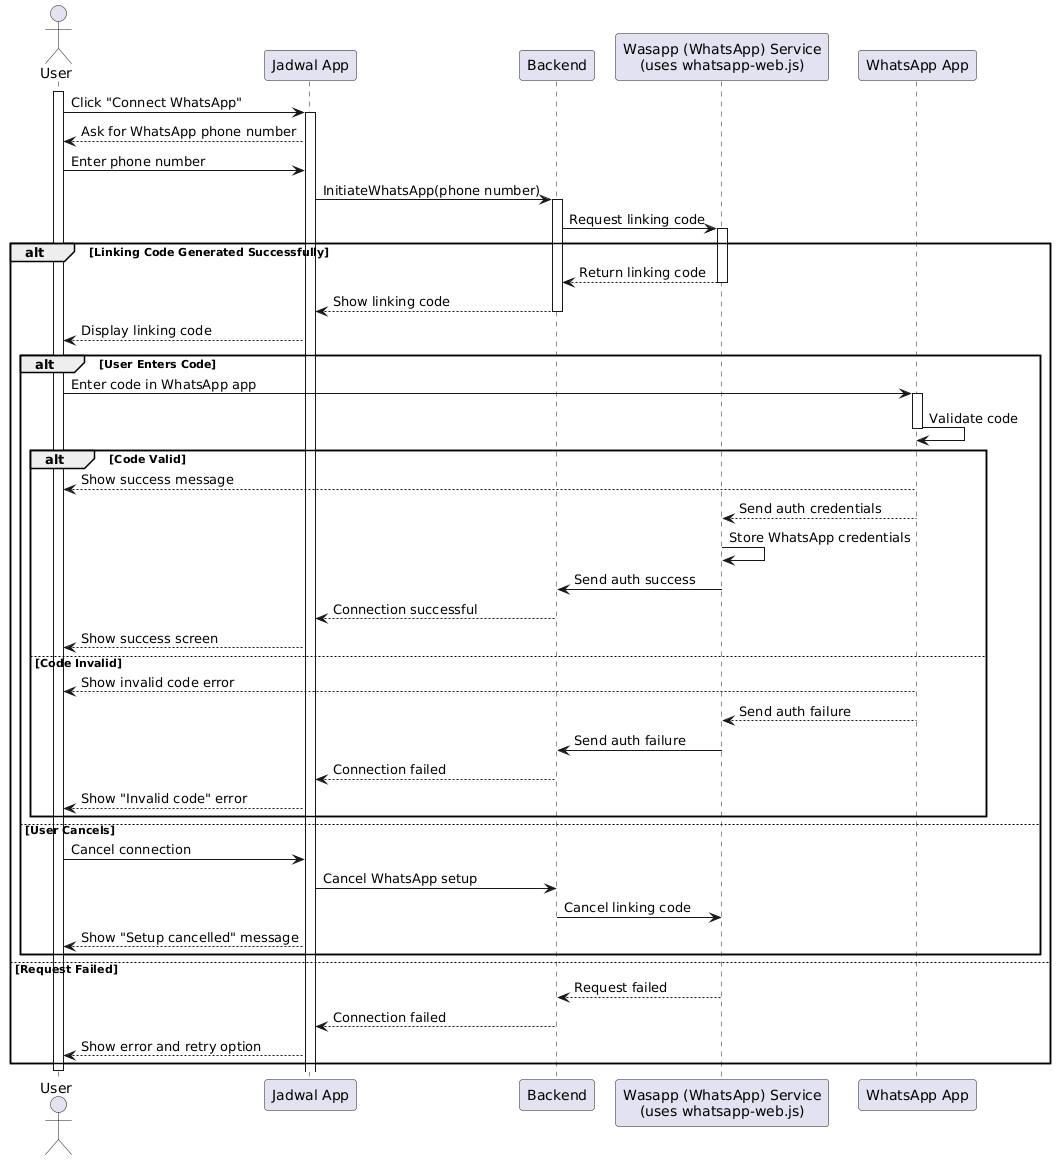
\includegraphics[width=\textwidth]{images/docs/diagrams/sequence-diagrams/all-sequence-diagrams/Connect WhatsApp.png}
  \caption{Connect WhatsApp Sequence Diagram}
  \label{fig:seq/connect-whatsapp}
\end{figure}

The "Connect WhatsApp Sequence Diagram", shown in \textbf{Figure~\ref{fig:seq/connect-whatsapp}}, illustrates the two-phase authentication process for connecting a user's WhatsApp account to Jadwal. The sequence begins with the InitiateWhatsApp gRPC call, where the user provides their phone number to the Backend.

The Backend then communicates with the WhatsApp service to request a linking code. This interaction follows two possible paths:

\begin{itemize}
  \item If the linking code request succeeds:
        \begin{enumerate}
          \item The user receives the linking code in their WhatsApp application
          \item The user initiates the CompleteWhatsApp gRPC call with the linking code
          \item The Backend validates the code with WhatsApp
          \item Upon successful validation, the WhatsApp authentication credentials are securely stored in the Database for future use
        \end{enumerate}
  \item If the linking code request fails:
        \begin{itemize}
          \item The Backend immediately returns an InitiateWhatsApp failure response to the user
        \end{itemize}
\end{itemize}

During the completion phase, if the linking code validation fails, the Backend returns a CompleteWhatsApp failure response, requiring the user to restart the process. This secure two-phase authentication ensures that only legitimate WhatsApp account owners can connect their accounts to Jadwal while maintaining the integrity of the WhatsApp integration.
\begin{usecase}{Continue with Google}
  \ucbasicinfo{\#2}{HIGH}{Regular}
  \ucshortdescription{This UC allows users to login or continue with Google if we have a Google account}
  \uctrigger{This UC starts when the user enters their email to the system.}
  \ucactors{User}{Google}
  \ucpreconditions{User must have an activated or valid Google email.}
  \ucrelationships{Send Welcome Email}{N/A}{N/A}
  \ucinputsoutputs{
    \begin{itemize}
      \item \textbf{Google account} (Source: User)
      \item \textbf{Authentication request to Google} (Source: System)
    \end{itemize}
  }{
    \begin{itemize}
      \item \textbf{Success or error message} (Destination: User)
      \item \textbf{Authentication response} (Destination: Google)
    \end{itemize}
  }
  \ucmainflow{
    \begin{enumerate}
      \item The user click continue with Google.
        \ucinfo{System displays "continue with Google" button}
      \item Authentication request.
        \ucinfo{A request sent to Google for user authentication and get JWT and sent it to the system, while the system will generate a our JWT}
      \item Authentication response.
        \ucinfo{Confirmation of successful authentication}
    \end{enumerate}
  }
  \ucalternateflows{
    \begin{itemize}
      \item User cancels authentication
      \item Authentication failure
    \end{itemize}
  }
  \ucexceptions{
    \begin{itemize}
      \item Invalid Google email
      \item Network issue
    \end{itemize}
  }
  \ucconclusion{}
  \ucpostconditions{The user is successfully authenticated and redirected to the main application interface}
  \ucbusinessrules{
    \begin{itemize}
      \item User should have valid Google account
    \end{itemize}
  }
  \ucspecialrequirements{Sign-in page should display clear button and error message}
\end{usecase}
\begin{usecase}{Set Event Priority}
    \ucbasicinfo{HIGH}{Regular}
    \ucshortdescription{The user adds or modifies an event, and the system detects a conflict with an existing event in the calendar.}
    \uctrigger{The user adds or modifies an event, and the system detects a conflict with an existing event in the calendar.}
    \ucactors{User}{None}
    \ucpreconditions{The user is logged into the application}
    \ucrelationships{Send Welcome Email}{N/A}{N/A}
    \ucinputsoutputs{
      \begin{itemize}
        \item \textbf{Conflicting events (both the new event and the existing event)} (Source: User)
        \item \textbf{Priority decision} (Source: User)
      \end{itemize}
    }{
      \begin{itemize}
        \item \textbf{The system prioritizes the selected event based on the user's choice
       } (Destination:  Calendar)
        \item \textbf{Confirmation messages} (Destination: User Interface)
      \end{itemize}
    }
    \ucmainflow{
      \begin{enumerate}
        \item Conflict Detection
          \ucinfo{The system detects overlapping events and prompts the user with a conflict}
        \item Choose Priority Option  
          \ucinfo{The system displays a dialogue box with both conflicting events and asks the user to select which event should take priority.}
        \item Resolve Conflict
          \ucinfo{The system offers options to either reschedule the lower-priority event or keep both events with a conflict warning}
        \item Save
          \ucinfo{•	After the user selects the priority, the system saves the decision, either reschedules the lower-priority event or marks it as conflicting and updates the calendar accordingly.}
      \end{enumerate}
    }
    \ucalternateflows{
      \begin{enumerate}
        \item User clicks on a date on the calendar to bring up a popup with event fields and the date is pre-filled. 
        \item The user can add a different color for the events
      \end{enumerate}
    }
    \ucexceptions{
      \begin{itemize}
        \item	No Available Time Slots 
      \end{itemize}
    }
    \ucpostconditions{The conflicting events are resolved, and the calendar reflects the user’s decision on which event to prioritize.}
    \ucspecialrequirements{The user interface must clearly show conflict warnings.}
    \ucconclusion{The use case ends when the user’s priority decision is saved, and the conflicting events are either rescheduled or maintained with a conflict warning.}
\end{usecase}
\begin{usecase}{Schedule Prayer Times}
    \ucbasicinfo{High}{Regular}
    \ucshortdescription{Allows users to create, edit, and manage their prayer time schedules.}
    \uctrigger{User selects the option to schedule prayer times.}
    \ucactors{User}{None}
    \ucpreconditions{User must be logged into the system.}
    \ucrelationships{N/A}{N/A}{N/A}
    \ucinputsoutputs{
      \begin{itemize}
        \item \textbf{User's prayer time details} (Source: user)
        \item \textbf{(date, time)}
      \end{itemize}
    }{
      \begin{itemize}
        \item \textbf{Confirmation of scheduled prayer times, calendar entries.}
      \end{itemize}
    }
    \ucmainflow{
      \begin{enumerate}
        \item User navigates to the prayer scheduling page.
          \ucinfo{User is presented with a form to enter prayer times. Display of the scheduling interface.}
        \item User inputs prayer time details.
          \ucinfo{Input fields for time, date, and prayer type. User's input is captured for validation.}
        \item User saves the schedule.
          \ucinfo{System checks for valid input. Confirmation message displayed.}
        \item System confirms schedule creation.
          \ucinfo{User receives a notification. Scheduled prayer times are saved in the system.}
      \end{enumerate}
    }
    \ucalternateflows{
      \begin{itemize}
        \item If input is invalid, display error messages.
      \end{itemize}
    }
    \ucexceptions{
      \begin{itemize}
        \item If there's a system error, display a relevant error message.
      \end{itemize}
    }
    \ucpostconditions{The system generates calendar entries for the scheduled prayer times.}
    \ucspecialrequirements{The system must support notifications for prayer times.}
    \ucconclusion{User's prayer times are successfully scheduled.}
    \ucbusinessrules{
      \begin{itemize}
        \item Prayer times must be within valid time ranges.
      \end{itemize}
    }
\end{usecase}

% Bibliography
\bibliography{references}
\bibliographystyle{apalike}

\end{document}